  \section{基于$k$-CBP~的碰撞检测算法}
    
      \subsection{$k$-CBP~间的相交测试}
      \begin{frame}
        \frametitle{}
        \begin{block}{AABB树法}
          将生成的$k$-CBP视为普通的三角形,实现简单,适用于模型较小的静止碰撞检测场景。
        \end{block}
        \begin{block}{GJK法}
          计算凸多面体之间的最近距离的~GJK~算法\footfullcite{bergen1999fast}。\\
          Minkowski~差,即~$\mathbb{A} - \mathbb{B} = \{ \bm{a} - \bm{b} | \bm{a} \in \mathbb{A}, \bm{b} \in \mathbb{B}\} $。
GJK~算法的核心思想在于若两个凸多边形相交,则凸多边形顶点的~Minkowski~差所围成的多边形必包含原点,因为若~$\mathbb{A}$~和
~$\mathbb{B}$~相交即~$\mathbb{A}$~和~$\mathbb{B}$~必含有公共交集,
即至少含有一点同时属于~$\mathbb{A}$~和~$\mathbb{B}$~,该点的~Minkowski~差即为原点~$\bm{O}(0, 0)$。
        \end{block}

        \note{
          基于k-CBP的碰撞检测问题,首先要解决k-CBP间的相交测试,有下面两种方法:\\
          一是将k-CBP视为普通的三角网格模型,用传统AABB树方法进行相交检测。\\
          二是利用计算凸体之间最近距离的GJK算法。该算法利用了Minkowski(闵可夫斯基)差的概念。核心思想在于若两个凸多边形相交,则凸多边形顶点的~Minkowski~差所围成的多边形必包含原点。
        }
      \end{frame}

      \begin{frame}
        \frametitle{二维~GJK~算法示例}
        \begin{figure}[htbp]
        \subfloat[相交]{
          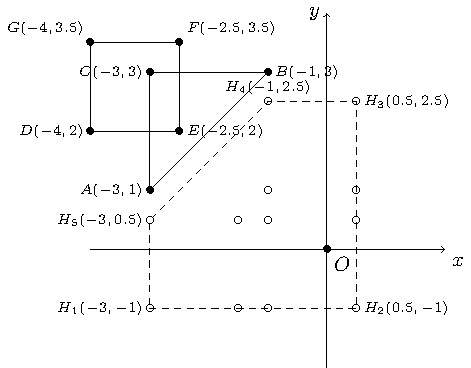
\includegraphics[width=.48\textwidth,page=1]{gjkExample.pdf}
        } 
        \subfloat[不相交]{
          \includegraphics[width=.48\textwidth, page=2]{gjkExample.pdf}
        }
        \end{figure}
        
        \note{
          以两个例子来说明,左图四边形和三角形相交,其Minkowski差围成的多边形H1H2\ldots H5就包含原点。而右边的不相交,其Minkowski差围成的多边形不包含原点。
        }
      \end{frame}

      \frame{
        \frametitle{GJK~算法}
        \vspace{-2em}
         \begin{columns}[onlytextwidth]
          \begin{column}{0.46\textwidth}
              \begin{figure}[htbp]
          \hspace{-9em}
              \subfloat%[第一步]
              {
                \includegraphics[width=.65\textwidth,page=3]{gjkExample.pdf}
              }\\ \vspace{-3em}\hspace{3em}
              \subfloat%[不相交]
              {
                \includegraphics[width=.65\textwidth, page=4]{gjkExample.pdf}
              }\\ \vspace{-2em} \hspace{-8em}
              \subfloat%[不相交]
              {
                \includegraphics[width=.65\textwidth, page=5]{gjkExample.pdf}
              }
             \end{figure}
          \end{column}
          \begin{column}{1.05\textwidth}
            \vspace{-2em}
            \scalebox{0.5}
            {
              \begin{minipage}{\textwidth}
                \begin{algorithm}[H]
                \caption{基于~GJK~的~$k$-CBP~相交检测算法}
                \label{alg:gjk}
                \begin{algorithmic}[1]
                \Require
                两个~$k$-CBP~$k\texttt{-}CBP_1, k\texttt{-}CBP_2$
                \Ensure
                ~$k$-CBP~是否相交
                \Function{KCBPDetectionBasedOnGJK}{$k\texttt{-}CBP_1, k\texttt{-}CBP_2$}
                    \State $\bm{d} \gets \Call{initNormal}$
                    \State $\bm{D} \gets \Call{Support}{k\texttt{-}CBP_1, k\texttt{-}CBP_2, \bm{d}}$
                    \State $S \gets \{p\}$
                    \State $iter \gets 1 , \bm{d} \gets -\bm{d}$
                    \While{$inter++ < MaxIter$}
                        \State $\bm{D} \gets \Call{Support}{k\texttt{-}CBP_1, k\texttt{-}CBP_2, \bm{d}}$
                        \If {$\bm{D} \cdot \bm{d} < 0 $}
                            \State \Return \textbf{False}
                        \EndIf
                        \State $S \gets S \cup \bm{D}$
                        \State $ contains \gets \Call{CheckContainUpdate}{S, \bm{d}}$ \Comment{检测是否包含原点,对集合~$S$~进行规约,并获取下一次迭代的方向~$\bm{d}$}
                        \If {$contains$}
                            \State \Return \textbf{True} \Comment{包含原点,直接返回相交,否则继续迭代}
                        \EndIf
                    \EndWhile
                    \State \Return \textbf{False} \Comment{达到最大迭代次数,根据需求返回相交或者不相交}
                \EndFunction
                \end{algorithmic}
                \end{algorithm}
              \end{minipage}
          }
          \end{column}
        \end{columns}
        
        \note{
          接下来就是怎样判断Minkowski差包含原点。GJK算法是一个迭代算法,刚开始取一个方向计算该方向上的支持点(Minkowski差围成多边形沿该方向的投影点),\\
          通过上一步的结果计算下一步迭代方向,如左图(鼠标操作)第一个支持点D1,下一次迭代找到D2,第三次迭代D3,此时D1D2D3就包含了原点。
        }
      }

      \subsection{三角形间的相交测试}
      \frame{
        %\frametitle{}
            \vspace{-0.5em}
            \begin{figure}[htbp]
              \centering
                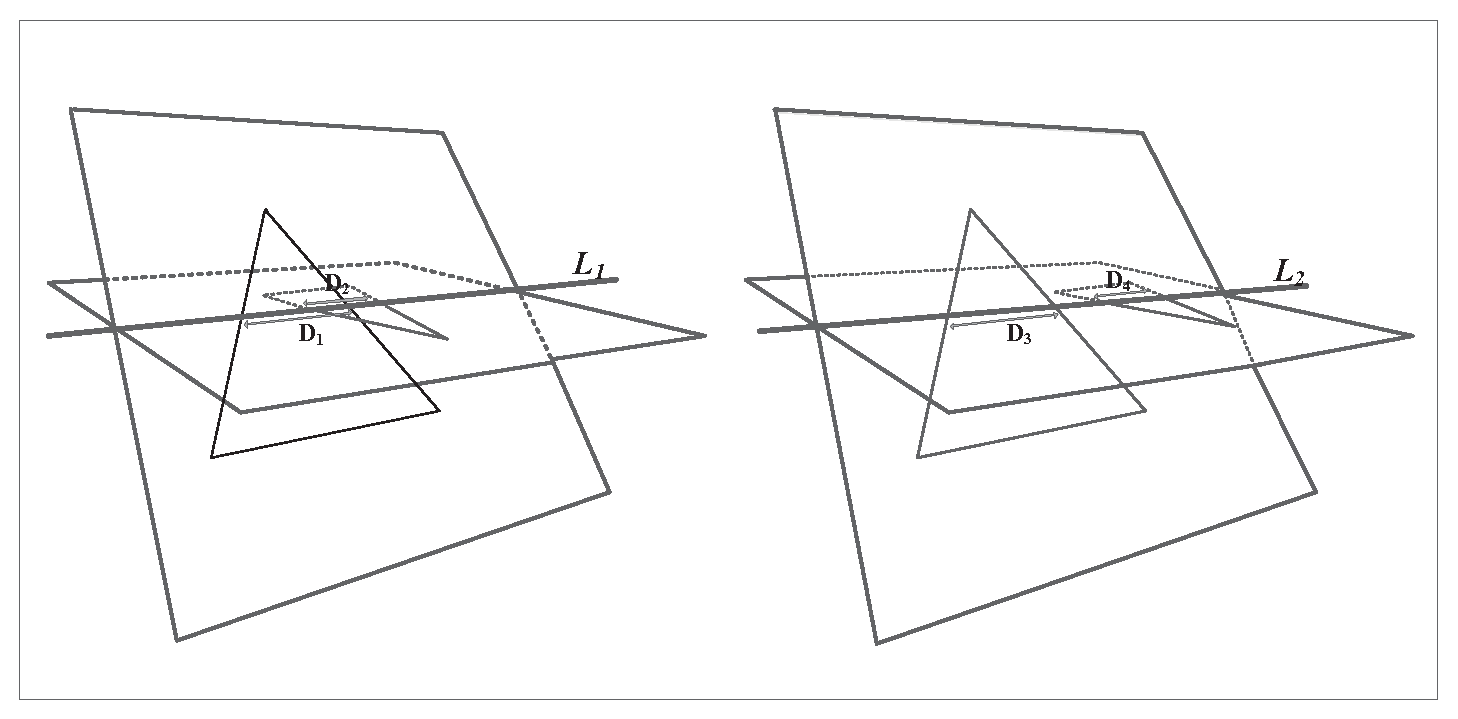
\includegraphics[width=3.0in]{TriangleTriangleTest.eps}
                \caption{两个非共面三角形的位置关系}
              \label{fig:two:triangle:ui}
            \end{figure}
            \vspace{-1.0em}
          \scriptsize 
          三角形~$T_1,T_2$坐标~$\Rightarrow$平面方程$\Pi_1,\Pi_2$$\Rightarrow$~$T_2$~到~$\Pi_1$~的有向距离~$\bm{l}_{1i}, i \in \{1,2,3\}$\footfullcite{Moller1997}:
          \begin{enumerate}[(1)]
            \item 若~$\forall i \in \{1,2,3\}, l_{1i} = 0$,即三角形~$T_2$~的三个顶点到三角形~$T_1$~所在~$\Pi_1$~的距离都为$0$,则两个三角形共面;$\Rightarrow$ 共面三角形求交。
            \item 若~$\forall i \in \{1,2,3\}, l_{1i} > 0$ 或~$\forall i \in \{1,2,3\}, l_{1i} < 0$,即三角形~$T_2$~的三个顶点到三角形~$T_1$~所在~$\Pi_1$~的有向距离同号,则~$T_2$~在~$\Pi_1$~的同一侧,可立即排除相交;
            \item 其他,三角形~$T_2$~必交~$\Pi_1$~于一条线段。$\Rightarrow$判断两个区间线段$D_1,D_2$是否相交。
          \end{enumerate}
         
          \note{
            三角形的相交测试也较简单。因为三角形三个点坐标已知,可推出平面方程,进而得到点到另一个平面的有向距离,根据有向距离分3种情况。(1)\ldots(2)\ldots (3)转化为投影到公共交线的区间线段是否相交。
          }
      }

      \subsection{基于$k$-CBP~的碰撞检测算法}

        \frame{
          \frametitle{$k$-CBP的有效性}
            \begin{figure}
            \centering
            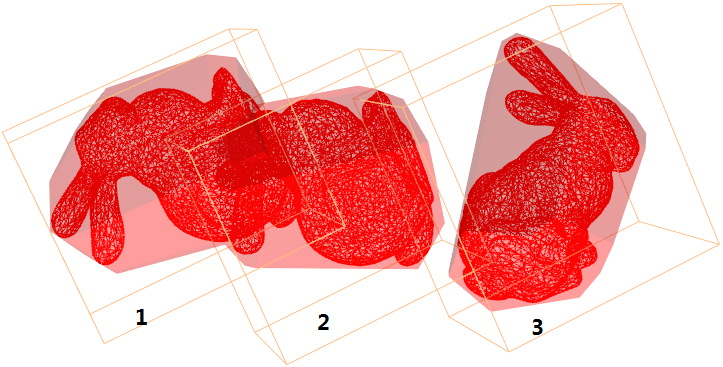
\includegraphics[width=2.5in]{figures/bunny-box-kcbp-collsion-detection-example.png}
            \caption{~$k$-CBP~应用于碰撞检测示例}
            \label{lbl:bunny-box-kcbp-collsion-detection-example}
            \end{figure}

            \footnotesize 图中模型~1~与~2、2~与~3~的包围盒分别相交, 而其~$16$-CBP~仅~1~与~2~相交, 实际模型仅~1~与~2~相交。 
            \note{
            这个例子展示了将k-CBP应用于碰撞检测的有效性。图中模型~1~与~2、2~与~3~的包围盒分别相交, 而其~$16$-CBP~仅~1~与~2~相交, 实际模型仅~1~与~2~相交。 
            }
        }
        \frame{
          \frametitle{静止场景碰撞检测算法} 
          \vspace{-2em}
          \begin{figure}[htpb]
            \centering
            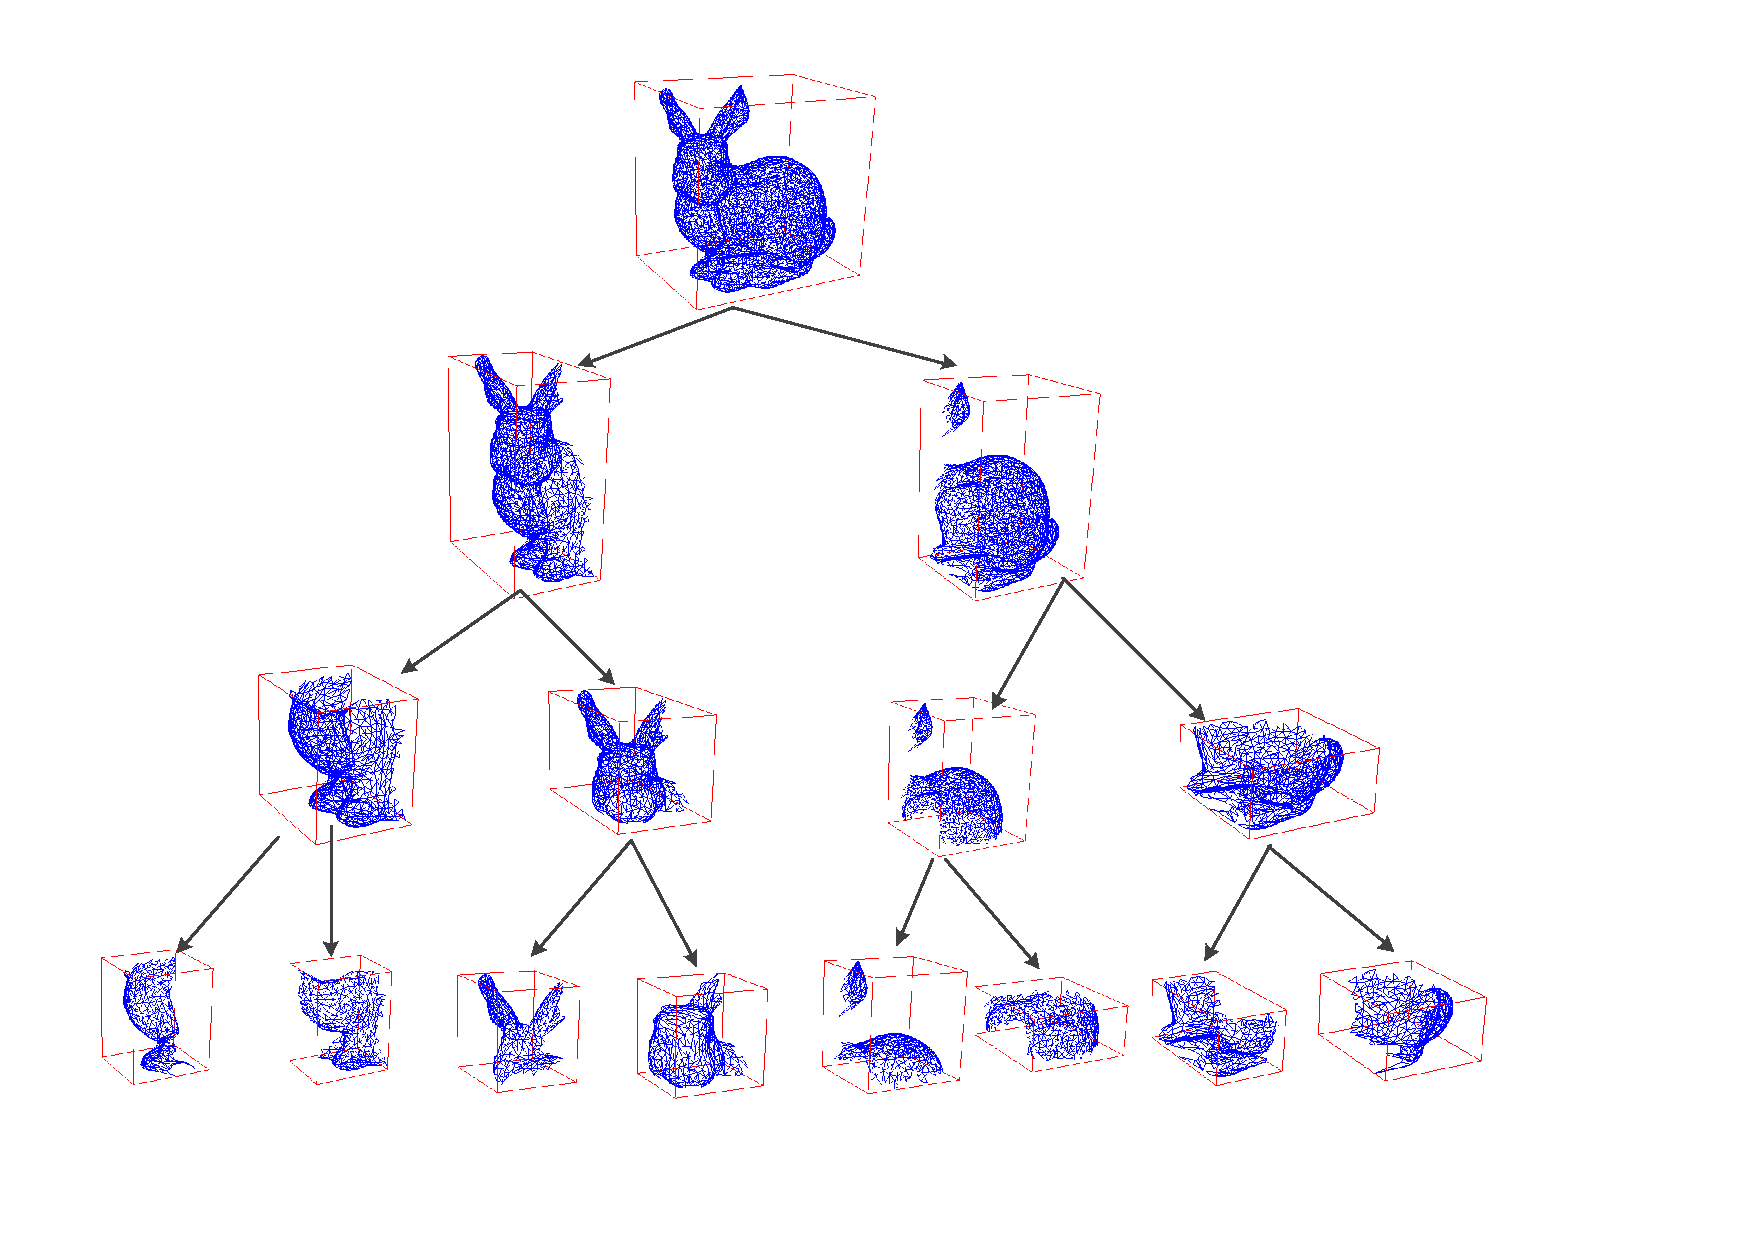
\includegraphics[width=0.5\textwidth]{bunny-aabb-bvh-4-layers.pdf}
            \caption{Bunny~模型的~AABB~树形结构(部分)\href{./bv-bunny.gif}{\beamergotobutton{动态图}} } %adobe pdf reader can open it in browser
            \label{fig:bunny:aabb:bvh:toplayer4}
          \end{figure} 
          \vspace{-1em}
           \begin{figure}[htpb]
              \centering
              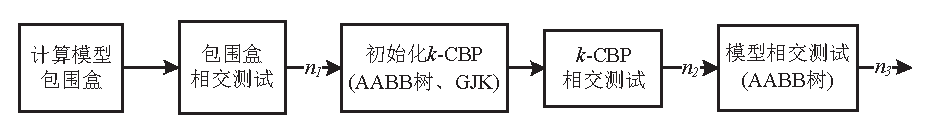
\includegraphics[width=\textwidth]{collision-detection-flowchart.eps}
              \caption{基于~$k$-CBP~的碰撞检测算法流程图}
              \label{fig:flowchart:cd}
            \end{figure} 
          
            \note{
            这是Bunny模型的AABB树结构,【看动态图】,静止场景下基于k-CBP的碰撞检测算法流程图如图17所示。
            }
        }
          \frame{
          \frametitle{运动场景碰撞检测算法} 
          \begin{columns}[onlytextwidth]
           \begin{column}{0.35\textwidth}
           \begin{figure}[H]
            \hspace{-4em}
            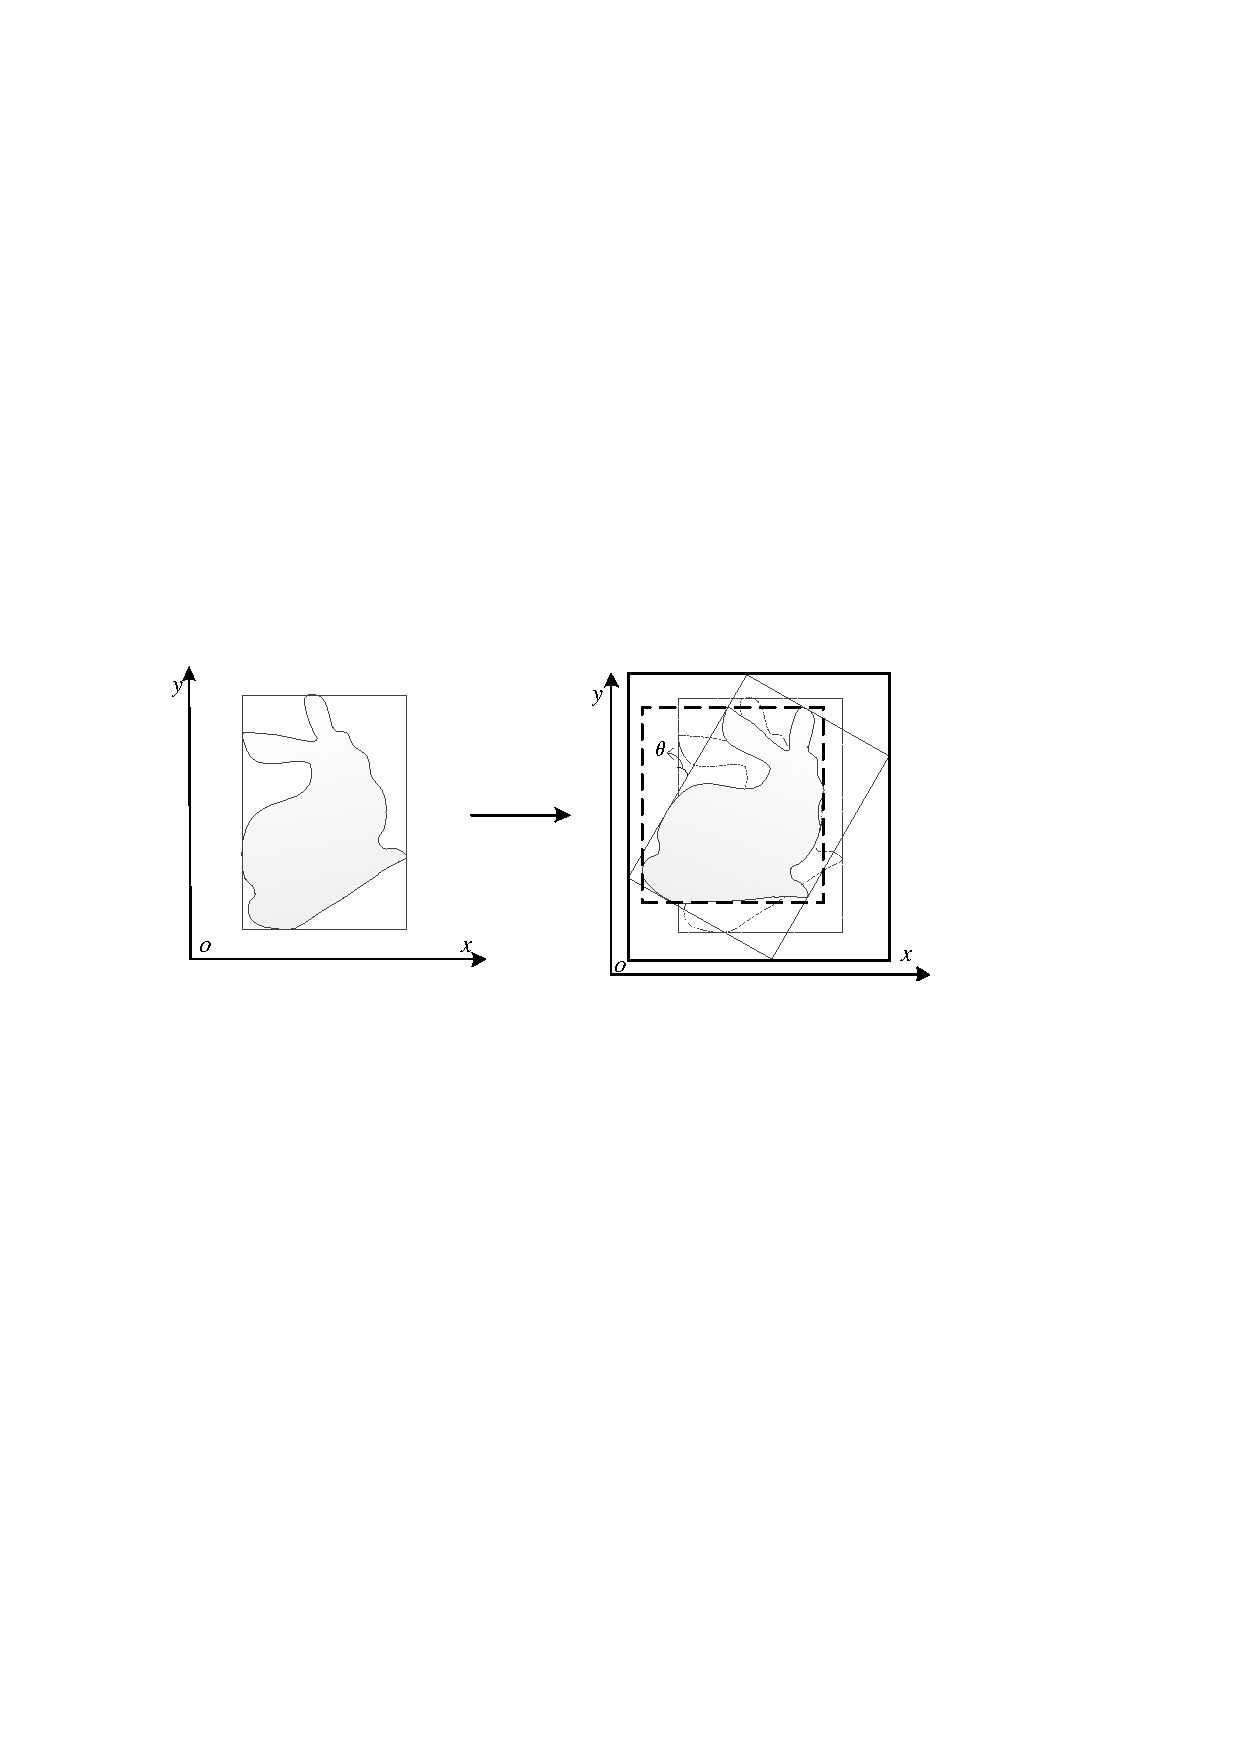
\includegraphics[width=2.5in]{bunny-2d-AABB-Moving.pdf}
            \caption{\tiny AABB~更新策略图}
            \label{fig:bunny:moving}
          \end{figure}
          \scriptsize
          将变换矩阵$\bm{M}=\bm{R}(\bm{n}, \theta) \cdot \bm{T}(\bm{t})$ \\
          应用于GJK顶点、AABB顶点。
          \end{column}
          \begin{column}{0.95\textwidth}
          \begin{figure}[htbp]
            \centering
            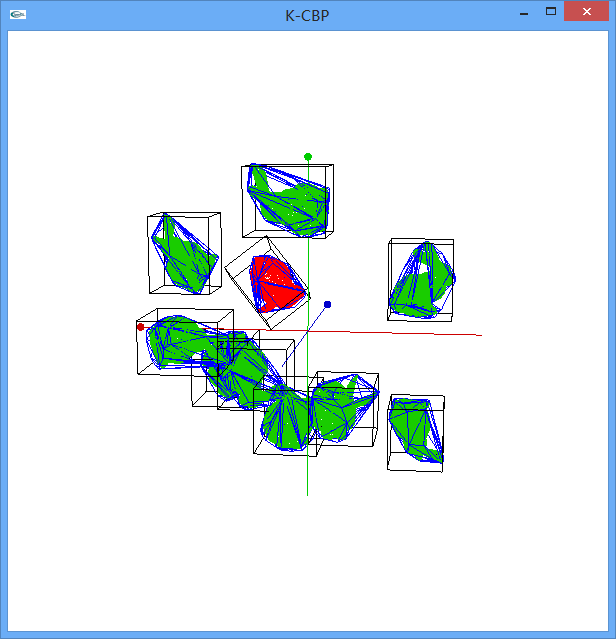
\includegraphics[width=1.8in]{dynamic-bunny-m10-sA1.png}
            \caption{运动场景碰撞检测示例\href{./cd-bunny.gif}{\beamergotobutton{动态图}}}
            \label{fig:bunny:moving}
          \end{figure}
          %\animategraphics[controls, buttonsize=3mm, width=1.8in]{10}{bvh-bunny-origin/bvh-bunny-}{0}{9} % 不靠谱
          \end{column}
          \end{columns}

          \note{
            运动场景下需要将变换矩阵应用到GJK顶点上,AABB更新时采取了一种近似策略,原先包围盒的8个顶点算出新的包围盒。图19是一个运动场景的示例,其中一个模型运动,运动过程中与其他所有模型进行相交检测。【看动态图】
          }
        }

    \subsection{实验结果及分析}

    \frame{
      \frametitle{实验结果:$k$-CBP~用于碰撞检测的有效性}
       \begin{table}[htbp]
         \tiny
      \caption{$k$-CBP~和包围盒应用于碰撞检测结果对比}
      \label{tab:exp:box:kcbp:collsiondetection}
      \centering
      \begin{tabular}{lccccccc}
       \toprule[1.5pt]
       \multirow{2}{*}{$n$} & CT(Box) & CT($16$-CBP) & DT(Box) & DT($16$-CBP) & $r$(Box) & $r$($k$-CBP) & DP(Model)\\ %\multirow{2}{*}{DP(Model)} \\
                            & (ms)    & (ms)          & (ms)  & (ms)          & (\%)      & (\%)  & (对)  \\
        \midrule[1.0pt]
         10 & 0.1 & 1.8 &    26.0  & 0.1    & 0.00  & 100.00 & 0\\
         30 & 0.2 & 2.9 &   134.0  & 70.0   & 45.45 & 83.33 & 5\\
         50 & 0.5 & 4.8 &   506.0  & 255.2  & 46.34 & 86.36 & 19 \\
         70 & 0.4 & 4.8 &   901.1  & 492.5  & 44.16 & 80.95 & 34 \\
         90 & 0.7 & 5.7 &  1324.0  & 734.7  & 41.82 & 73.02 & 46 \\
        100 & 0.7 & 7.8 &  1481.0  & 870.7  & 43.31 & 75.34 & 55 \\
        150 & 1.0 & 9.8 &  4153.1  & 2473.0 & 42.98 & 70.75 & 150 \\
        200 & 1.6 & 12.8 & 8049.3  & 4430.9 & 41.02 & 71.32 & 281 \\
        \bottomrule[1.5pt]
       \end{tabular}
      \end{table}
        \scriptsize 其中模型和凸包围多面体是否相交都采用了~AABB~树的方式进行判断。

        \note{
          先用一个实验说明k-CBP用于碰撞检测的有效性。不能说因为用了kCBP,反而比直接用包围盒更慢了。表中n为场景中模型数量,CT为构造时间,DT为场景中碰撞检测时间,r为命中率即模型实际相交数量/包围体相交数量。 
        }
    }

  %  \frame{
  %    \frametitle{实验结果:不同包围体对比}
  %    \vspace{-2em}
  %      \begin{figure}[htbp]
  %        \hspace{-4em}\subfloat[包围体构造时间]
  %      {
  %        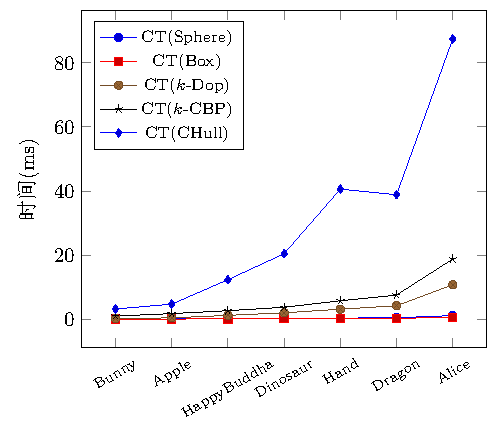
\includegraphics[width=.40\textwidth,page=1]{bvprebench.pdf}
  %      }\hspace{-1.6em}
  %      \subfloat[包围体命中率]
  %      {
  %        \includegraphics[width=.40\textwidth, page=3]{bvprebench.pdf}
  %      }\hspace{-1.6em}
  %      \subfloat[初始化时间]
  %      {
  %        \includegraphics[width=.40\textwidth, page=6]{bvprebench.pdf}
  %      }\hspace{-1.6em}
  %     \end{figure} 
  %     \vspace{-1em}
  %     \scriptsize 构造时间上基本满足:$\textnormal{凸包} > k\textnormal{-CBP} > k\textnormal{-DOP} > \textnormal{Sphere} \approx  \textnormal{Box}$,
  %     包围体命中率基本满足:$\textnormal{凸包} > k\textnormal{-CBP} > k\textnormal{-DOP} > \textnormal{Box} > \textnormal{Sphere}$。紧致程度和包围体的命中率满足正相关关系。

  %     \note{
  %      这个实验是对不同包围体进行了比较。左是构造时间,中为碰撞检测的命中率,右为碰撞检测初始化时间(包括了构造包围体时间和AABB树时间),命中率低的需要初始化模型数量更多因此初始化时间更长。
  %      紧致程度和包围体的命中率满足正相关关系。 // 碰撞检测时间PPT中省略,因为碰撞检测算法一致,没有明显差别。
  %     }
  %  }

    \frame{
      \frametitle{实验结果:静止场景与$k$-DOP树对比}
      \vspace{-2em}
        \begin{figure}[htbp] 
        \hspace{-3em}
        \subfloat[\tiny Bunny(4968个三角形)\label{fig:exp:static:bunny}]
        {  
           \includegraphics[width=0.35\textwidth,page=3]{staticcd.pdf}
        }\hspace{-1.0em}
        \subfloat[\tiny Apple(8040个三角形)\label{fig:exp:static:apple}]
        {  
            \includegraphics[width=0.35\textwidth, page=4]{staticcd.pdf}
        }\hspace{-1.0em}
        \subfloat[\tiny HappyBuddha(50000个三角形)\label{fig:exp:static:happyBuddha}]
        {  
           \includegraphics[width=0.35\textwidth, page=14]{staticcd.pdf}
        }%\hspace{-2.0em}
        \caption{静止场景下本文算法与基于~$k$-DOP~树算法实验结果对比($k=24$)}
        \label{fig:chart:exps:kdop:kcbp:k24}
        \end{figure}
        \vspace{-1em}
        \scriptsize 基于~$k$-DOP~树\footfullcite{abenchmarking2007}算法的碰撞检测库\href{http://cgvr.cs.uni-bremen.de/research/colldet/}{\beamergotobutton{CollDet}}~是Gabriel Zachmann~等人实现的。
        \note{
          这是与基于k-DOP树的算法在静止场景下的对比。坐标轴Y轴左边标的是初始时间,右边是碰撞检测时间,横坐标为模型数量。红线和蓝线为初始化时间。\\
          从中可以看出,模型较小时,三种算法碰撞检测时间差不多,模型变大,本文基于GJK的算法优势就体现出来了。
        }
    }
  %   \frame{
  %    \frametitle{实验结果:静止场景与$k$-DOP树对比}
  %    \vspace{-2em}
  %     \begin{figure}[htbp] 
  %        \centering
  %        \subfloat[Bunny(4968个三角形)\label{fig:exp:static:k24:k46:bunny}]
  %        {  
  %           \includegraphics[width=0.45\textwidth,page=12]{staticcd.pdf}
  %        }
  %        \subfloat[HappyBuddha(50000个三角形)\label{fig:exp:static:k24:k46:happybuddha}]
  %        {  
  %            \includegraphics[width=0.45\textwidth, page=18]{staticcd.pdf}
  %        }
  %        \caption{静止场景下不同~$k$~值实验结果对比}
  %        \label{fig:chart:exp:kdop:kcbp:k24:k46}
  %    \end{figure}
  %  \note{可能时间不够,不同k值的比较省略了}
  %  }

     \frame{
      \frametitle{实验结果:运动场景与$k$-DOP树对比}
      \vspace{-2em}
         \begin{figure}[htbp] 
          \hspace{-4em}
          \subfloat[\tiny Bunny(4968个三角形)\label{fig:exp:dynamic:m10:bunny}]
          {  
             \includegraphics[width=0.4\textwidth,page=7]{dynamiccd.pdf}
          }\hspace{-1.7em}
          \subfloat[\tiny HappyBuddha(50000个三角形)\label{fig:exp:dynamic:m10:happyBuddha}]
          {  
             \includegraphics[width=0.4\textwidth, page=14]{dynamiccd.pdf}
          }\hspace{-1.7em}
          \subfloat[\tiny Hand(128314个三角形)\label{fig:exp:dynamic:m10:hand}]
          {  
             \includegraphics[width=0.4\textwidth, page=16]{dynamiccd.pdf}
          }\hspace{-2.0em}
          \caption{运动场景下本文算法与基于~$k$-DOP~树算法实验结果对比($k=24,n=10$)}
          \label{fig:chart:exps:kdop:kcbp:k24:m10:dynamic}
          \end{figure} 
          
          \note{
            这是运动场景下的对比结果,横坐标为运动的次数,纵坐标为运动相应次数碰撞检测所耗费的时间。\\
            可以看出,随着模型变大,基于AABB的算法跟k-DOP树算法差距越来越小,而基于GJK的算法优势明显。
          }
    }
    
  %  \frame{
  %    \frametitle{实验结果:运动场景与$k$-DOP树对比}
  %    \vspace{-2em}
  %       \begin{figure}[htbp] 
  %  \centering
  %  \subfloat[Bunny(4968个三角形)\label{fig:exp:static:k24:k46:bunny:dynamic}]
  %  {  
  %     \includegraphics[width=0.45\textwidth,page=11]{dynamiccd.pdf}
  %  }
  %  \subfloat[HappyBuddha(50000个三角形)\label{fig:exp:static:k24:k46:happybuddha:dynamic}]
  %  {  
  %      \includegraphics[width=0.45\textwidth, page=18]{dynamiccd.pdf}
  %  }
  %  \caption{运动场景下不同~$k$~值实验结果对比}
  %  \label{fig:chart:exp:kdop:kcbp:k24:k46:dynamic}
  %  \end{figure} 
  %  }
